%%%%%%%%%%%%%%%%%%%%%%%%%%%%%%%%%%%%%%%%%%%%%%%%%%%%%%%%%%%%%%%%%%%%%%%%
%    INSTITUTE OF PHYSICS PUBLISHING                                   %
%                                                                      %
%   `Preparing an article for publication in an Institute of Physics   %
%    Publishing journal using LaTeX'                                   %
%                                                                      %
%    LaTeX source code `ioplau2e.tex' used to generate `author         %
%    guidelines', the documentation explaining and demonstrating use   %
%    of the Institute of Physics Publishing LaTeX preprint files       %
%    `iopart.cls, iopart12.clo and iopart10.clo'.                      %
%                                                                      %
%    `ioplau2e.tex' itself uses LaTeX with `iopart.cls'                %
%                                                                      %
%%%%%%%%%%%%%%%%%%%%%%%%%%%%%%%%%%
%
%
% First we have a character check
%
% ! exclamation mark    " double quote  
% # hash                ` opening quote (grave)
% & ampersand           ' closing quote (acute)
% $ dollar              % percent       
% ( open parenthesis    ) close paren.  
% - hyphen              = equals sign
% | vertical bar        ~ tilde         
% @ at sign             _ underscore
% { open curly brace    } close curly   
% [ open square         ] close square bracket
% + plus sign           ; semi-colon    
% * asterisk            : colon
% < open angle bracket  > close angle   
% , comma               . full stop
% ? question mark       / forward slash 
% \ backslash           ^ circumflex
%
% ABCDEFGHIJKLMNOPQRSTUVWXYZ 
% abcdefghijklmnopqrstuvwxyz 
% 1234567890
%
%%%%%%%%%%%%%%%%%%%%%%%%%%%%%%%%%%%%%%%%%%%%%%%%%%%%%%%%%%%%%%%%%%%
%

%AIP Reprint Class%%%%%%%%%%%%%%%%%%%%%%%%%%%%%%%%%%%%%%%%%%%%%%%%%%%%%%%%%%%%%%%%%%%%%%%%%%%%%
\documentclass[aip,prl,amsmath,amssymb,reprint,superscriptaddress]{revtex4-1} %preprint version
\usepackage{graphicx}% Include figure files
\usepackage{dcolumn}% Align table columns on decimal point
\usepackage{bm}% bold math
\usepackage{epstopdf}

    \renewcommand{\topfraction}{0.9}    % max fraction of floats at top
    \renewcommand{\bottomfraction}{0.8}    % max fraction of floats at bottom
    \setcounter{topnumber}{2}
    \setcounter{bottomnumber}{2}
    \setcounter{totalnumber}{4}     % 2 may work better
    \setcounter{dbltopnumber}{2}    % for 2-column pages
    \renewcommand{\dbltopfraction}{0.9}    % fit big float above 2-col. text
    \renewcommand{\textfraction}{0.07}    % allow minimal text w. figs
    \renewcommand{\floatpagefraction}{0.7}    % require fuller float pages
    \renewcommand{\dblfloatpagefraction}{0.7}    % require fuller float pages
    \setlength{\abovecaptionskip}{5pt}
    \setlength{\belowcaptionskip}{5pt}
    \setlength{\parskip}{0pt}
    \setlength{\textfloatsep}{5pt} 

%%%%%%%%%%%%%%%%%%%%%%%%%%%%%%%%%%%%%%%%%%%%%%%%%%%%%%%%%%%%%%%%%%%%%%%%%%%%%%%%%%%%%%%%%%%%%%%%%%

%IOP preprint class %%%%%%%%%%%%%%%%%%%%%%%%%%%%%%%%%%%%%%%%%%%%%%%%%%%%%%%%%%%%%%%%%%%%%%%%%%%%%%
%\documentclass[12pt]{iopart}
%\newcommand{\gguide}{{\it Preparing graphics for IOP journals}}
%Uncomment next line if AMS fonts required
%\usepackage{iopams}
%\usepackage{graphicx}
%\usepackage{epstopdf}  
%%%%%%%%%%%%%%%%%%%%%%%%%%%%%%%%%%%%%%%%%%%%%%%%%%%%%%%%%%%%%%%%%%%%%%%%%%%%%%%%%%%%%%%%%%%%%%%%%%
%Slava's inserts %%%%%%%%%%%%%%%%%%%%%%%%%%%%%%%%%%%%%%%%%%%%%%%%%%%%%%%%%%%%%%%%%%%%%%%%%%%%%%
%\usepackage{amsfonts}
%\usepackage{amssymb}

%\newcommand{\ptt}[1]{\frac{\partial#1}{\partial t}}
%\newcommand{\vvec}{\mathbf{v}}
%\newcommand{\Bvec}{\mathbf{B}}
%\newcommand{\Evec}{\mathbf{E}}
%\newcommand{\Jvec}{\mathbf{J}}
%\newcommand{\Avec}{\mathbf{A}}
%%%%%%%%%%%%%%%%%%%%%%%%%%%%%%%%%%%%%%%%%%%%%%%%%%%%%%%%%%%%%%%%%%%%%%%%%%%%%%%%%%%%%%%%%%%%%%%%%%

\begin{document}
\title{Spatial correlations in a turbulent MHD laboratory plasma}

\author{A. Wan}
\affiliation{Swarthmore College, Swarthmore, PA, USA}
\author{D.A. Schaffner}
\affiliation{Swarthmore College, Swarthmore, PA, USA}
\author{V.S. Lukin}
\affiliation{Space Science Division, Naval Research Laboratory, Washington, DC, USA}
\author{W.H. Matthaeus}
\affiliation{Bartol Research Institute and Department of Physics and Astronomy, University of Deleware, Newark, DE, USA}
\author{M.R. Brown}
\affiliation{Swarthmore College, Swarthmore, PA, USA}
\date{\today}
\begin{abstract}
Correlation analysis is used to determine the Taylor microscale and magnetic Reynolds number in a turbulent laboratory MHD plasma.  We find that radial correlation length is shorter for a colliding MHD wind tunnel plasma than for a single plume.  An unambiguous measure of the magnetic Reynolds number is estimated from the Taylor microscale and the correlation scale, then compared to a calculation using the Spitzer resistivity.
\end{abstract}

\maketitle

\section{Introduction}



Two point velocity correlation functions have been measured in conventional fluids for decades~\cite{frisch95,Belmabrouk98}, but two point magnetic spatial correlations in plasmas are less common.  The first proper two-point single time measurements of the magnetic correlation function in the solar wind plasma were performed by Matthaeus, et al \cite{Matthaeus05}.  They used simultaneous magnetic field data from several spacecraft, including the four Cluster spacecraft flying in tetrahedral formation.  Simultaneous measurements were performed with separations ranging from $150~km$ (using pairs of Cluster satellites) to $350~R_E$ ($2.2 \times 10^6~km$).  From measurements of the outer correlation scale, and the Taylor microscale, they report an effective magnetic Reynolds number of the solar wind $R_m^{eff}  = 230,000$.

In a set of follow-up papers, Weygand, et al \cite{Weygand07,Weygand09,Weygand10,Weygand11} have modified and improved the earlier result.  In particular, they describe a method using fits of Cluster separations from 100 to $10^6~km$ \cite{Weygand07}, and extrapolating the Taylor microscale down to zero separation.  We discuss this method below.  These more detailed measurements confirm the earlier work  \cite{Matthaeus05} and find a solar wind magnetic Reynolds number of $R_m^{eff}  = 260,000 \pm 20,000$.  In addition, using data in the magnetospheric plasma sheet (tailward of Earth), they find a much smaller Reynolds number $R_m^{eff}  = 111 \pm 12$ since the outer correlation scale is much smaller in the plasma sheet.  Anisotropies in the correlation function parallel and perpendicular to the local magnetic field were studied in separate papers \cite{Weygand09,Weygand10}, with longer correlation lengths measured parallel to the local field.  Variations with solar wind speed were also studied \cite{Weygand11}.

This paper presents the first measurements of spatial correlation function in a high beta ($\beta \sim 0.1$), high Mach ($M \sim 0.4$) turbulent laboratory plasma in the wind-tunnel configuration of the Swarthmore Spheromak Experiment. The Taylor microscale and Taylor Reynolds number of this turbulent plasma is computed from these spatial correlation functions. The values for the a magnetic Reynolds number, $R_{m}$, computed using the Taylor Reynolds number, compares well to values of $R_{m}$ calculated using an estimation of the Spitzer resistivity from electron temperature measurements. These numbers can be compared to similar quantities found in space plasma observations or {\it in-situ} measurements from satellites. An example of the advantage of laboratory experiment in such turbulent research is given through a comparison of the spatial correlation functions in single plume versus colliding plume plasmas. The results indicate that colliding or merging plasma have a slightly smaller Taylor microscale than single plume or non-merging plasmas.

\section{Theory and Techniques}

A useful measure of fully developed turbulence is the spatial correlation function.  For a magnetohydrodynamic (MHD) plasma, the radial correlation function of the magnetic field can be written
%
\begin{equation}
R(r) =  \langle {\bf b(x) \cdot b(x + r)} \rangle
\label{eq:correlation1}
\end{equation}
%
where {\bf b} is the fluctuating part of a turbulent magnetic field (${\bf B}(x, t) = {\bf B_0 + b}$).  For well-behaved turbulence, the magnetic fluctuations at two points should become uncorrelated at large spatial separation and the correlation function should vanish ($R \rightarrow 0$ as $r \rightarrow \infty$).  

The magnetic Taylor microscale, $\lambda_{T}$, can be formally defined as
%
\begin{equation}
\lambda_T^2 = \frac{\langle {\bf b}^2 \rangle}{\langle (\nabla \times {\bf b})^2 \rangle}.
\label{eq:tayscale}
\end{equation}
%
This definition identifies the Taylor microscale as the scale associated with mean square spatial derivatives of the fluctuating magnetic field $\bf{b}$. A similar definition of the Taylor microscale in conventional fluids involves spatial derivatives of the fluctuating velocity field~\cite{frisch95}. It is at this scale that one would expect dissipation effects to become important, although actual dissipation likely occurs at smaller, kinetic scales~\cite{Mattaeus08} ($k_D \lambda_T = R_m^{1/4}$).  We expect that the Taylor microscale should be on the order of but larger than the Larmor scale ($\rho_i \approx 1~mm$ in the SSX wind tunnel) and the ion inertial scale ($c/\omega_{pi} \approx 5~mm$ in SSX). For small values of $\lambda_{T}$, the correlation function can be approximated as
%
\begin{equation}
R(r) \approx  \langle b^2 \rangle \left(1 - \frac{r^2}{2 \lambda_T^2}  \right)
\label{eq:correlation2} 
\end{equation}
%
Thus, we arrive at the measurement of the Taylor microscale in the paper by fitting a parabolic function of the form in Equation~\ref{eq:correlation2} to our measured spatial correlation functions. For these fits, we can use an between 3 and 16 separate points. By separately fitting a parabola to the spatial correlations for different numbers of points, a plot of Taylor microscale as a function of number of fit points is constructed. This curve is then extrapolated to intersect with the y-axis which represents the Taylor microscale at zero separation. This value is taken as the Taylor microscale for the turbulence.

Then, a Taylor Reynolds number can be written~\cite{frisch95}
%
\begin{equation}
R_{mT}  = \left(\frac{\lambda_{C}}{\lambda_T} \right)^2
\label{eq:RM-eff}
\end{equation}
%
which is related to the actual magnetic Reynolds number
%
\begin{equation}
R_m  = \left( R_{mT} \right) ^2 .
\label{eq:RM-eff2}
\end{equation}
%
where, $\lambda_{C}$, is the correlation scale. This scale, $\lambda_{C}$, is less formally defined and represents the scale over which the correlation of fluctuations reaches some level. Often, the integral scale, defined as
%
\begin{equation}
\lambda_{I}  = \frac{1}{\langle b^2 \rangle} \int_0^\infty R(r) dr
\label{eq:tayscale2}
\end{equation}
%
can be used, but can be problematic when $R(r)$ does not approach zero. In this paper, three versions of a correlation length are given: one, uses the integral scale definition, but only after fitting the $R(r)$ to a Gaussian function and using this fit function in Equation~\ref{eq:tayscale2}. A second form uses the measured spatial correlation function directly, and determines the length $r_{l}$ at which $R(r_{l})=0.5$. A third form is to just take the radius of the wind-tunnel, $r_{wt} = 7.75cm$ which represents the true physical limit of the correlation function. From these values of the correlation length, estimates of the Taylor Reynolds number and magnetic Reynolds number are made using Equations~\ref{eq:RM-eff} and~\ref{eq:RM-eff2}. These can be compared to a computation of the magnetic Reynolds number derived by evaluation of the Spitzer conductivity,$\sigma_{SP}$,
\begin{equation}
R_m = \mu_0 V \sigma_{SP} L.
\label{eq:RM-calc} 
\end{equation}
%
where $\sigma_{SP}\sim T_{e}^{-3/2}$. Using $T_e = 10~eV$ for the SSX wind tunnel, and $V=20km/s$, the Spizter magnetic Reyonlds number ranges between 118 and 236 depending on whether the outer scale, L, is taken as the radius (7.75cm) or the diameter (15.5cm) of the wind-tunnel.
%An equivalent formulation of the Taylor scale in terms of the spectrum is
%
%\begin{equation}
%\frac{1}{\lambda_T^2}  = \int_0^\infty dk k^2 E(k)/\int_0^\infty dk E(k)
%\label{eq:tayscale3}
%\end{equation}
%
%The Fourier transform of the correlation function is the spatial energy spectrum, $E(k)$:
%
%\begin{equation}
%E(k) = \frac{1}{2 \pi} \int_0^L e^{ikr} R(r) dr
%\label{eq:spectrum1}
%\end{equation}
%
%We can compare a measurement of the energy spectrum $E(k)$ to the Fourier transform of the measured correlation function $R(r)$.

\section{Experimental Apparatus}

\begin{figure}[!htbp]
\centerline{
\includegraphics[width=8.5cm]{Images/simulation_diagram_radcorr_paper}}
\caption{\label{fig:chamber} Diagram showing orientation of plasma, plasma gun source, and 16 channel, 3-axis magnetic pick up coil. The probe extends radially into the plasma at the midplane. Blue lines represent simulation generated magnetic field lines of the plasma.}
\end{figure}

%\textsf{TODO: Need some standard experiment setup description. Plasma production, lab info? Definitely need to talk about the magnetic probes: tri-directional $\dot{B}$ probes inserted radially at the mid-plane of the flux conserver. Measures change in magnetic field at 16 points along radius.}
The measurements are made on the MHD wind-tunnel configuration of the Swarthmore Spheromak Experiment. Plasma guns located on both sides of a 15.5 diameter, 86cm long cylindrical copper tube produce highly magnetized, dense plasma ($B\sim 5kG, n\sim 1\times 10^{15} cm^{-3}$) using a plasma gun source. The turbulence is generated as the initial plasma structure (called a spheromak) undergoes a tilt-instability and expands into the copper tube or MHD wind-tunnel. Details of the formation process are discussed in previous work on SSX~\cite{schaffner14a,schaffner14b}. Magnetic fluctuations are recorded by a 16-channel, 3-axis, single-loop pickup coil probe located at the midplane and protruding radially into the cylindrical chamber. The measurement points span a region from about 1cm off the cylindrical axis to the inner edge of the chamber and are spaced by about 0.46cm. The coils measure fluctuations in $dB/dt$ using a 14-bit, 65MHz Dtaq digitizer and then numerically intergrated to construct $B(t)$ timeseries for each loop axis aligned in cylindrical coordinate directions: $B_{r}$, $B_{\theta}$, and $B_{z}$.

The data presented here is comprised of two configurations. The first has only one gun producing a single plasma plume. The second has both guns producing oppositely directed plasma plumes which collide and merge. The merging plumes are produced with opposite magnetic helicity. Data analyzed from each configuration consists of at least forty shots to create an ensemble average. The spatial correlation functions are constructed using a time range of $40$ to $60\mu s$ after the initial discharge. This time frame constitutes the most epoch of stationary fluctuations balanced between source and dissipation. 

%\textsf{TODO get Slava's description here? Relevant details such as the paradigm used (Hall/MHD), etc...}}
The experimental data is also compared to Hall-MHD simulated versions of the wind-tunnel plasma generated using the HiFi framework~\cite{schaffner14a} of both single plume and colliding plasma setups. The simulation data consisted of magnetic field measured along 8 equally-spaced radii at the midplane of the simulated flux conserver. The epoch used was $43-53 \mu s$, chosen to capture fluctuations in the simulated $B$-field that qualitatively resembled the $40-60\ \mu s$ epoch of the experimental data. 

%\textsf{TODO: need to try different epochs of the simulation data.

\section{Results}

Figure~\ref{fig:brbtbz} shows a scatter plot of spatial correlation values for $B(t)$ for each of the three probe directions. Each marker in the plot represents a single correlation coefficent between two probe points of a given separation; consequently, the number of points for each separation decreases as the separation length increases. There are $16-n$ points for a $n$ tip separation. The darkened data points indicate which points were used in plotting the fit equation \eqref{eq:correlation2}. Apart from providing a visual representation of experimental spread in data, this method also reveals locational variations in the correlation function that persist over multiple shots. For example, in Fig.\ \ref{fig:brbtbz}(b), it appears that there are two clusters of data, one with a generally higher correlation strength than the other. The higher correlation strength points correspond to tips further from the wall of the flux conserver; that this pattern is apparent after an averaging of 75 sets of data suggests that $B_\theta$ correlation strengths are influenced by wall proximity. Fig.\ \ref{fig:brbtbz}(b) shows how the parabolic fit \eqref{eq:RM-eff} can be applied to a subset of the data --- in this case the fit shown was performed only on the averaged correlation strengths from the four outer probe tips.

Figure~\ref{fig:brbtbz} shows contrast amongst the three directions of magnetic field. The $B_r$ field is highly correlated throughout, while in contrast the $B_z$ correlation strengths are highly scattered and less suggestive of any distinctive pattern. Though the fields in the plasma are completely dynamical---that is, there is no guide field---the direction of the magnetic field vector is for any given moment, typically in the $B_{r}$ direction. The noticeable difference in correlation functions observed, then, is suggestive of an anistropy between correlation lengths parallel and perpendicular to the mean field. However, it is prudent to focus on the correlation strengths of the $B_\theta$ signal, which are well-clustered and exhibit a sharper decay in correlation strength, thus giving a more precise measurement of the Taylor microscale $\lambda_T$. We proceeded to compare the correlation strengths of $B_\theta$ from merging and relaxation configurations of SSX with corresponding simulations. 

\begin{figure}[!htbp]
\centerline{
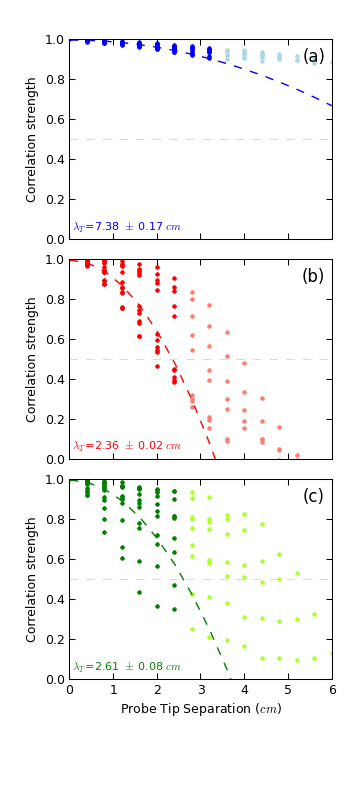
\includegraphics[width=8.5cm]{Images/brbtbz-081413.png}}
\caption{Single plume correlation functions for magnetic field in the (a) $\hat{r}$, (b) $\hat{\theta}$, (c) $\hat{z}$ directions}
\label{fig:brbtbz}
\end{figure}

Figure~\ref{fig:comparisons}(a) compares the spatial correlation functions from the single plume and colliding plume configurations of the experiment. The steeper decay of the merging configuration correlation function is indicative of a more turbulent plasma during the sampled epoch, which is intuitively expected. The parabolic fits are made to the first five points for each curve and the extracted Taylor scales also reflect the steeper slope of the merging versus single plume correlation function. Figure~\ref{fig:comparisons}(b) shows a comparison of the experimental single plume data to its single plume simulation counterpart. The shapes of the correlation functions are comparable within a few cm, but the simulation curve clear is steeper. The close correspondence at small separation distances results in a fairly close computed Taylor scale.

%While the two correlation curves look qualitatively different, it is enlightening that the radii of curvature (i.e.\ the curve obtained by fitting \eqref{eq:RM-eff}) obtained from experiment and from simulation are close. \textsf{mini-conclusion?} 

Figure~\ref{fig:comparisons}(c) presents results from the merging configuration and its simulation counterpart. Unlike the single plume comparison, these two curves have distinctly different shapes; in addition, the simulation curve is shallower than the experimental. This may be due the nature of the simulation at the midplane where the plumes are precisely meeting while it is not know exactly where the plumes meet in the experimental version. Using measurements slightly offset from the midplane of the simulation could imitate the variability in the merging plane of lab plasmas.
%The contrast between the laboratory and simulated results motivates deeper consideration of details of the simulation that differ from an experimental setup. One potential source of differences between the two is that the simulated plasmas always merge exactly at the midplane, and thus exactly where the measurements of $B$-field are obtained. 

\begin{figure}[!htbp]
\centering
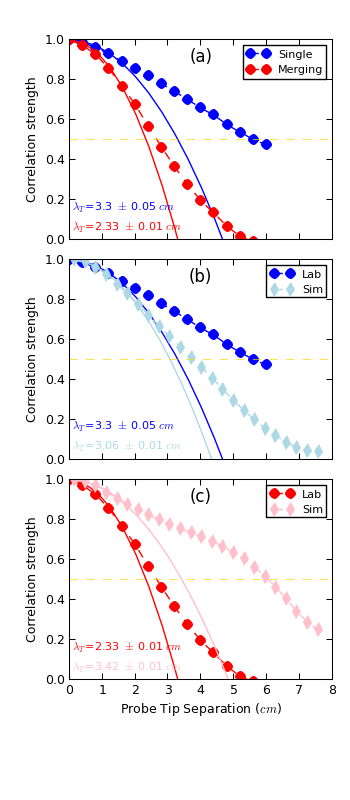
\includegraphics[width=8.5cm]{Images/comparisons.png}
\caption{\label{fig:comparisons} (a) Single vs.\ Merging. (b) Single, Lab vs.\ Sim. (c) Merging, Lab vs.\ Sim.}
\end{figure}

As shown in Figures \ref{fig:brbtbz} and \ref{fig:comparisons}, \eqref{eq:RM-eff} can be fitted to functions of correlation strength to obtain a value for the Taylor microscale $\lambda_T$. 
Following the example of Matthaeus et al.\cite{Matthaeus05}, we vary the number of points in the correlation function used in the fit and plot value of $\lambda_{T}$ extracted as a function of point number as shown in Fig.~\ref{fig:ndf}. Since the approximation for the Taylor microscale is calculated in the limit of zero-separation, the curves in Fig~\ref{fig:ndf} can be fit with a linear function in order to extrapolate the value of $\lambda_{T}$ at zero separation. to a zero-point fit. We take this value of $\lambda_{T}$ as the most physically accurate possible value of the Taylor microscale.
%(\textsf{TODO check the corresponding section in Bill's paper and use their language}) 

\begin{figure}[!htbp]
\centerline{
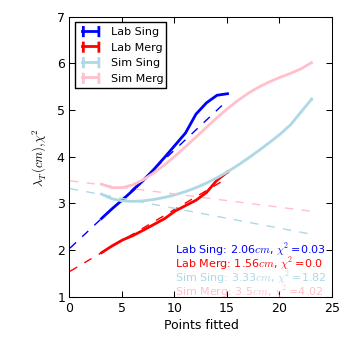
\includegraphics[width=0.5\textwidth]{Images/ndf.png}}
\caption{\label{fig:ndf} $\lambda_T$ vs. ndf. of parabola fit with error}
\end{figure}

Both the experimental single plume and colliding results show clear linearity in the trend. Fits to a linear function yield well-defined values of the Taylor microscale: $\lambda_T = 2.06cm$ for the relaxation configuration, and $\lambda_T = 1.56cm$ for the merging setup. The simulation curves, however, do not have clearly linear trends. The trends in $\lambda_{T}$ appears to begin fairly linear for larger numbers of fit points, but begin to flatten and even slightly curve up as the number of fit points decreases. This is due to some flattening of the correlation function near zero. If the inflected portions of the lines are ignored, extraplated values for zero-separation Taylor microscales appear to fall in the same range as the experiment. Note, however, that the single plume simulation appears to lie closer to the merging experiment than the single plume experiment. The overall merging correlation function also appears closer in shape to the single plume simulation. The merging simulation is the furthest again the furthest outlier.

Once this extrapolated $\lambda_T$ value has been obtained, calculating $R_m$ can be computed using one of the three values for $\lambda_{C}$. Table~\ref{tab:Rms1} displays the Taylor Microscale for each of the four datasets, along with the calculated Taylor Reynolds number computed using each form of $\lambda_{C}$: the integral scale, $\lambda_{I}$, the half-max scale, $r_{l}$, and the radius of the wind-tunnel, $r_{wt}$. Table~\ref{tab:Rms2} shows the computed values of the magnetic Reynolds number in comparison to the Spitzer conductivity computed $R_m$.

\begin{table} [htbp]
\caption{\label{tab:Rms1}Comparison of Taylor Microscale and Taylor magnetic Reynolds numbers for various cases.}
\begin{tabular}{ccccc}
\toprule
Dataset								& $\lambda_{T}$	&$R_{mT}(\lambda_{I})$&$R_{mT}(r_{l})$&$R_{mT}(r_{wt})$\\
\hline
Exp Single  					& 2.06 					& 7.8 								& 7.4						&14.1\\
Sim Single  					& 2.38 					& 1.7 								& 1.6						&10.6\\
Exp Merging 					& 1.56 					& 3.1 								& 3.2						&24.7\\
Sim Merging 					& 2.62 					& 9.7 								& 8.4						&8.7\\
\hline
\end{tabular}
\end{table}

\begin{table} [htbp]
\caption{\label{tab:Rms2}Comparison of Taylor Microscale and Taylor magnetic Reynolds numbers for various cases.}
\begin{tabular}{ccccc}
\toprule
Dataset								&$R_{m}(\lambda_{I})$&$R_{m}(r_{l})$&$R_{m}(r_{wt})$&$R_{m}(\sigma_{SP})$\\
\hline
Exp Single  					& 60.3 								& 54.6						&200					&118-236\\
Sim Single  					& 2.84 								& 2.73						&112					&118-236\\
Exp Merging 					& 9.6 								& 10.4						&609					&118-236\\
Sim Merging 					& 93.6 								& 70							&76.5					&118-236\\
\hline
\end{tabular}
\end{table}

This paper presents a measurement of the magnetic spatial correlation function of an MHD turbulent plasma in a laboratory setting. Comparison of different types of plasma in the machine shows that single plume plasma are slightly better correlated as a function of distance than merging plumes of plasma. The comparisons can be quantified by finding the zero-separation Taylor microscales for each plasma configuration which confirm the comparison of merging versus single plume. Moreover, the values found for the microscale are larger than any other length scale in these plasma at which dissipation effects might be expected to occur; this is in line with the typical interpretation of the Taylor microscale in fluid physics. The Taylor microscale has in turned been used to compute Taylor magnetic Reynolds number. These values compare fairly well to an estimate of the magnetic Reynolds number computed using Spitzer resistivity. Overall, the fact that the Reynolds number values are all $> 1$ show that the plasmas exhibit dissipation scales smaller than injection scales and likely have some (if short) inertial range physics. The method for measuring Taylor scales and Reynolds numbers in this way is shown to be applicable in an experimental device. Future work entails probing further how these scales change as plasma parameters are modified as well as much detailed comparison to space physics situations such as in the solar wind and the magnetosheath.

%\textsf{Sample calculation of $R_m$ values: ``w/ radius'' means using $\lambda_C = 7.8\ cm$ (?), ``w/ Int. Scale'' means performing the fit to find e-folding time (Talk about measuring correlation length: Gaussian/other fits), computed means using the formula for $R_m$ with Spitzer resistivity. Hopefully they all end up in the same ballpark. }

%Table \ref{tab:Rms} compares the magnetic Reynolds numbers obtained from four different data sets: experimental single-plume and merging configurations, and their corresponding simulations. It compares the values of $R_m$ obtained when the various $\lambda_C$ calculations are performed: the ``$R_m$ w/ Radius'' column uses the radius of the flux chamber as the correlation scale, $\lambda_C = 7.8\ cm$; the ``w/ Int. Scale'' performs the integration in \eqref{eq:tayscale2} to calculate the correlation scale. 

%These results are comparable to the magnetic Reynolds number calculated using \eqref{eq:RM-calc}, $R_M = 300$. 

%Any uncertainty in fitting \eqref{eq:correlation2} to the data is magnified when the ratio $\lambda_C/\lambda_T$ is raised to the fourth power. An estimate of the error in the Lab Single value of $R_m$ calculated using the radius is 
%
%\begin{equation}
%\Delta R_m = 4 (\dfrac{\Delta \lambda_T}{\lambda_T} + \dfrac{\Delta \lambda_C}{\lambda_C}) = 4 (\dfrac{0.054}{3.30} + \dfrac{0.1}{7.8})= 11.7\%
%\label{eq:error}
%\end{equation}
%
%\textsf{TODO is this the right way to estimate error?}



%The values obtained for the two configurations in the laboratory straddle the value of $R_m$ calculated from \eqref{eq:RM-calc}. This agreement (check error?) is BLAH --- \textsf{Something about how this method is cool because we were able to obtain a value for two physical parameters ($\lambda_T$ and $R_m$) just through a correlation analysis, which basically looks at turbulence/noise? Plus this method is useful for plasmas that we can't directly measure temperature for --- good alternative to the calculation with Spitzer resistivity.}


% ----------------------------------------------------------------
%\section*{Acknowledgements}
%We gratefully acknowledge many useful discussions with William Matthaeus. This work has been funded by the US DoE Experimental Plasma Research program and the National Science Foundation.  The %simulations were performed using the advanced computing resources (Cray XC30 Edison system) at the National Energy Research Scientific Computing Center.
% ----------------------------------------------------------------
\section*{References}
\begin{thebibliography}{99}

\bibitem{Belmabrouk98}
Belmabrouk, H., and M. Michard (1998), Taylor length scale measurement by laser Doppler velocimetry, Exp. Fluids, 25, 69Ð76.

\bibitem{Matthaeus05}
Matthaeus, W. H. and Dasso, S. and Weygand, J. M. and Milano, L. J. and Smith, C. W. and Kivelson, M. G., Phys. Rev. Lett. 95, 231101 (2005) Spatial Correlation of Solar-Wind Turbulence from Two-Point Measurements

\bibitem{Weygand07}
Weygand, J. M., Matthaeus, W. H., Dasso, S., Kivelson, M. G.,
and Walker, R. J. (2007), J. Geophys. Res., 112, A10201.

\bibitem{Weygand09}
Weygand, J. M., Matthaeus, W. H., Dasso, S., Kivelson, M. G.,
Kristler, L. M., and Mouikis, C. (2009), J. Geophys. Res., 114,
A07213.

\bibitem{Weygand10}
Weygand, J. M., Matthaeus, W. H., El-Alaoui, M., Dasso, S., and
Kivelson, M. G. (2010), J. Geophys. Res., textit115, A12250.

\bibitem{Weygand11}
Weygand, J. M., Matthaeus, W. H., Dasso, S., and Kivelson, M.
G. (2011), J. Geophys. Res., 116, A08120.

\bibitem{Matthaeus08}
Matthaeus W. H., Weygand, J. M., Chuychai, P., Dasso, S.,
Smith, C. W., and Kivelson, M. (2008), Astrophys. J., 678,
L141.

\bibitem{frisch95}Frisch, U. 1995, {\it Turbulence} (Cambridge: Cambridge Univ. Press)

\bibitem{schaffner14a} D.A. Schaffner {\it et al.} Turbulence analysis of an experimental flux rope plasma. {\bf 56} 064003 (2014).

\bibitem{schaffner14b} D.A. Schaffner {\it et al.} Observation of turbulent intermittency scaling with magnetic helicity in an MHD plasma wind-tunnel. Submitted to PRL? Feb 2014.

%\bibitem{sorrisovalvo99}Sorriso-Valvo, L. {\it et al.} Geophys. Res. Lett. {\bf 26}, 1801–1804 (1999).

%\bibitem{wan12}Wan, M. {\it et al.} ApJ. {\bf 744} 177 (2012).

%\bibitem{sorrisovalvo01}Sorriso-Valvo, L. {\it et al.} Planet. Space Sci. {\bf 49}, 1193–1200 (2001).

%\bibitem{marrelli05}Marrelli, L. {\it et al.} Phys. Plasmas. {\bf 12}, 030701 (2005).

%\bibitem{Greco08}A. Greco, P. Chuychai, W. H. Matthaeus, S. Servidio and P. Dmitruk, Intermittent MHD structures and classical discontinuities, Geophys. Res. Lett. {\bf 35}, L19111 (2008).

%\bibitem{Greco09}Greco, A., Matthaeus, W. H., Servidio, S., Chuychai, P., and Dmitruk, P.: Statistical Analysis of Discontinuities in Solar Wind ACE Data and Comparison with Intermittent MHD Turbulence, ApJ {\bf 691}, L111 (2009).

%\bibitem{Wan09}Wan, M., Oughton, S., Servidio, S., and Matthaeus, W. H.: Generation of non-Gaussian statistics and coherent structures in ideal magnetohydrodynamics, Phys. Plasmas {\bf 16}, 080703 (2009).

%\bibitem{Servidio11b}Servidio, S. {\it et al}, J. Geophys. Res. {\bf 116}, A09102 (2011).

%\bibitem{Gray13} T. Gray, M. R. Brown, and D. Dandurand. Phys. Rev. Lett. {\bf 110}, 085002 (2013). 

%\bibitem{schaffner14} D.A. Schaffner {\it et al.} Turbulence analysis of an experimental flux rope plasma. Submitted to Plas. Phys. Cont. Fusion. (2014).

%\bibitem{Taylor86} J. B. Taylor, Rev. Mod. Phys. {\bf 58}, 741 (1986).

%\bibitem{Matthaeus80} W.H. Matthaeus and D. Montgomery, Ann. N.Y. Acad. Sci. {\bf 357}, 203 (1980).

%\bibitem{torrence98}C. Torrence, G.P. Compo, A practical guide to wavelet analysis. Bull. Am. Meteorol. Soc. {\bf 79}, 6178 (1998).

%\bibitem{clauset09}A. Clauset, C. Rohilla Shalizi, M.E.J. Newman, Power-law distributions in empirical data, SIAM Rev. {\bf 51}, 661703 (2009).

%\bibitem{wan12}M. Wan, K. T. Osman, W. H. Matthaeus, and S. Oughton, Investigation of intermittency in magnetohydrodynamics and solar wind turbulence: scale-dependent kurtosis, ApJ {\bf 744}, 171 (2012).

%\bibitem{Gray10}T. Gray, V. S. Lukin, M. R. Brown, C. D. Cothran, Three-dimensional reconnection and relaxation of merging spheromak plasmas, Phys. Plasmas {\bf 17}, 102106 (2010).

%\bibitem{goldstein94}Goldstein, M.L., Roberts, D.A. and Fitch, C.A. Jour. Geo. Res. {\bf 99} 11519-11538 (1994).

%\bibitem{ji95}Ji, H., Prager, S.C. and Sarff, J.S. Phys. Rev. Lett. {\bf 74} 2945 (1995).

%\bibitem{telloni12}Telloini, D. {\it et al.}. ApJ. {\bf 751} 19 (2012).

%\bibitem{matthaeusVelli11}Matthaeus, W.H. and Velli, M. Space Sci. Rev. {\bf 160} 145-168 (2011).

%\bibitem{greco12}A. Greco {\it et al.} ApJ. {\bf 749} 105 (2012).

\end{thebibliography}

\end{document}

